\section{Увод}
Судоку је популарна загонетка са бројевима која се среће у многобројним дневним новинама  и часописима. Директан превод са јапанског имена ове загонетке је "јединствен број" што и осликава задатак ове игре, формирати квадратну матрицу димензија \(n \times n\) (најчешће 9х9) тако да се у свакој колони и врсти може затећи само једна појава бројева од 1 до \textit{n}. Исто правило примењује се и на одређене подматрице чије су димензије \(\sqrt{n} \times \sqrt{n}\). Играчу је на почетку игре дата матрица са неколико већ додељених вредности, а његов задатак је да матрицу попуни до краја, а да не прекрши правило јединствености појављивања бројева. Пример нерешене, а затим успешно решене загонетке може се видети на слици \ref{fig:unsolved_solved}.

\begin{figure}[H]
    \centering
    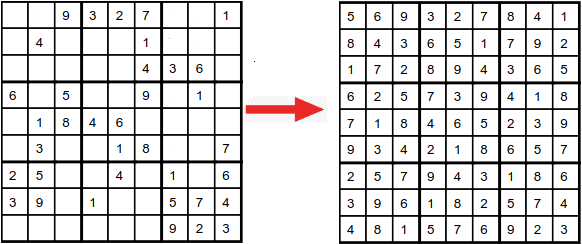
\includegraphics[width=1\textwidth]{images/unsolved_solved.png}
    \caption{Пример нерешеног и решеног судокуа}
    \label{fig:unsolved_solved}
\end{figure}

Циљ овог рада је паралелизација алгоритма за решавање ове загонетке. У даљим поглављима биће додатно појашњени основни појмови потребни за разумевање алгоритама, постојећа решења, а затим и ауторове имплементације овог алгоритма различитим приступима (\textit{openMP} примитиви и \textit{task}-ови, \textit{openMPI}), као и порeђење њихових перформанси.